\section{System Architecture and Methodology}
\label{sec:methodology}

\subsection{Pipeline Overview}
DeepPacket Analyzer decouples packet capture and parsing using a high-throughput, multi-threaded producer-consumer pipeline. As illustrated in Fig.~\ref{fig:arch}, incoming raw frames are ingested via Npcap or offline PCAP dumps and immediately enqueued onto a cache-aligned circular ring buffer.

\begin{figure}[htbp]
\centering
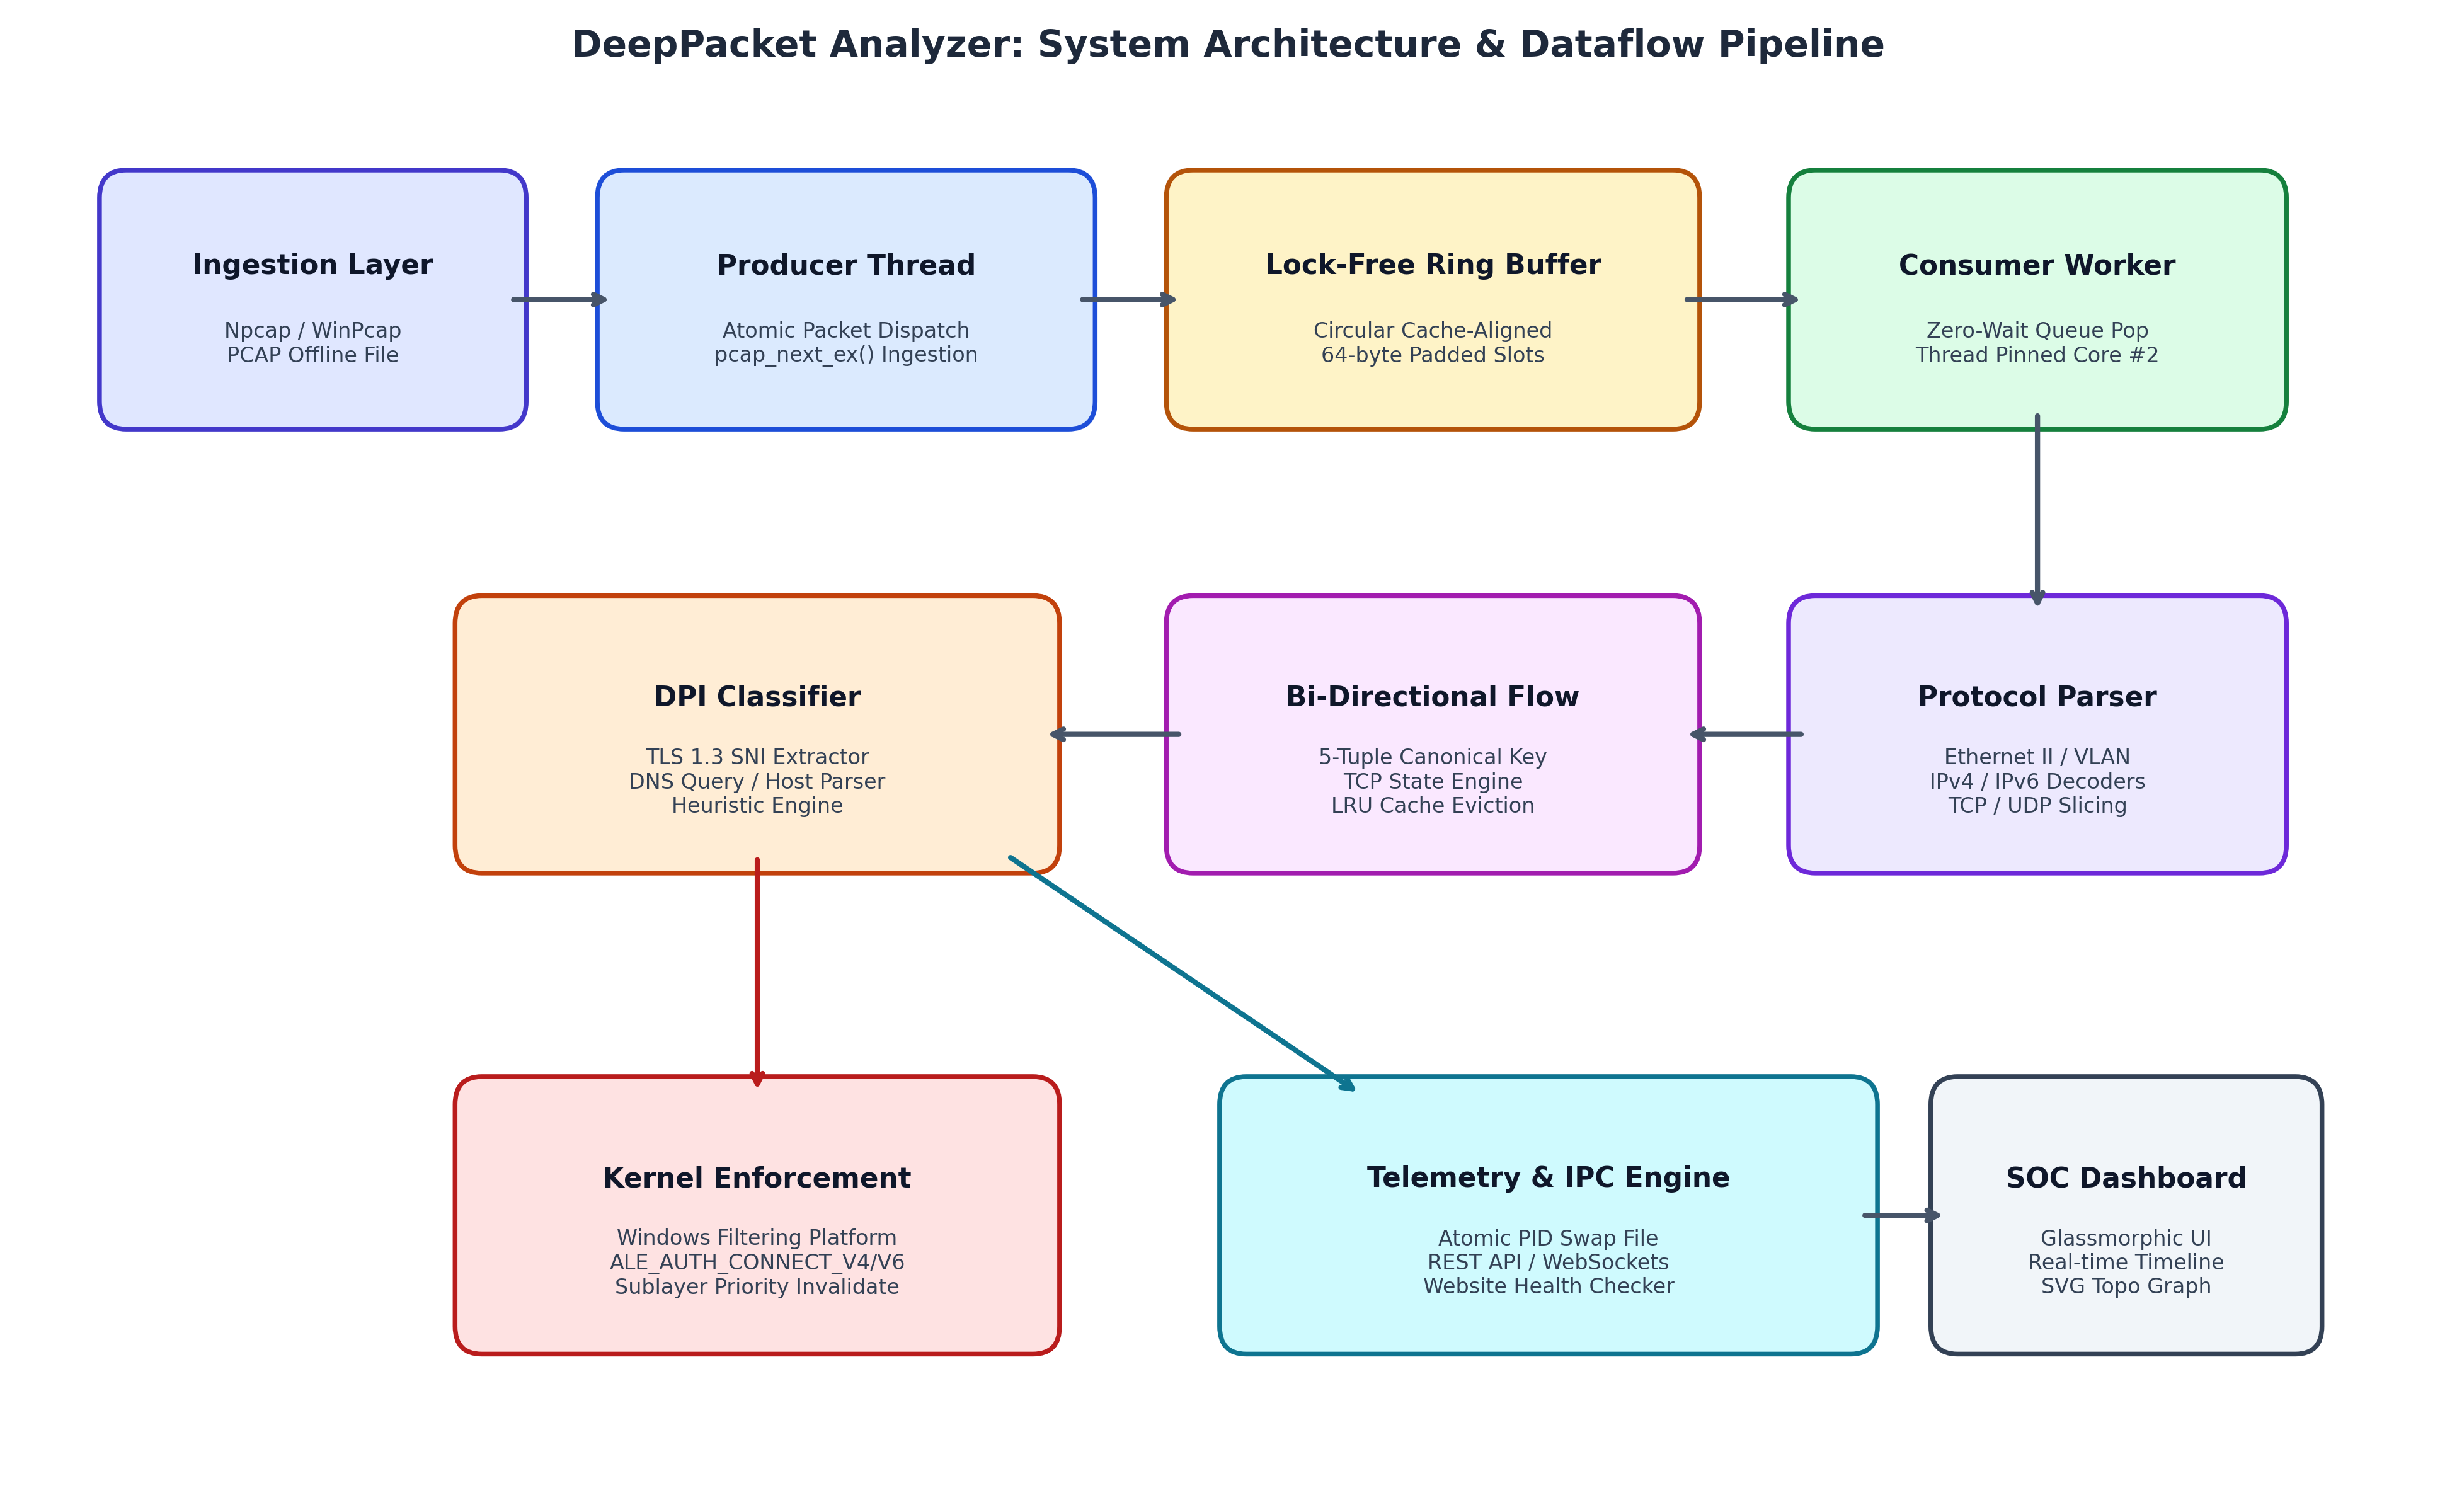
\includegraphics[width=\linewidth]{SystemArchitecture.png}
\caption{DeepPacket Analyzer End-to-End System Architecture.}
\label{fig:arch}
\end{figure}

\subsection{Decoupled Thread Pipeline}
To avoid packet dropouts during burst intervals, frame ingestion is isolated within a dedicated producer thread, while parsing, flow attribution, and deep protocol inspection are executed by worker threads pinned to isolated CPU cores (Fig.~\ref{fig:thread_pipeline}).

\begin{figure}[htbp]
\centering
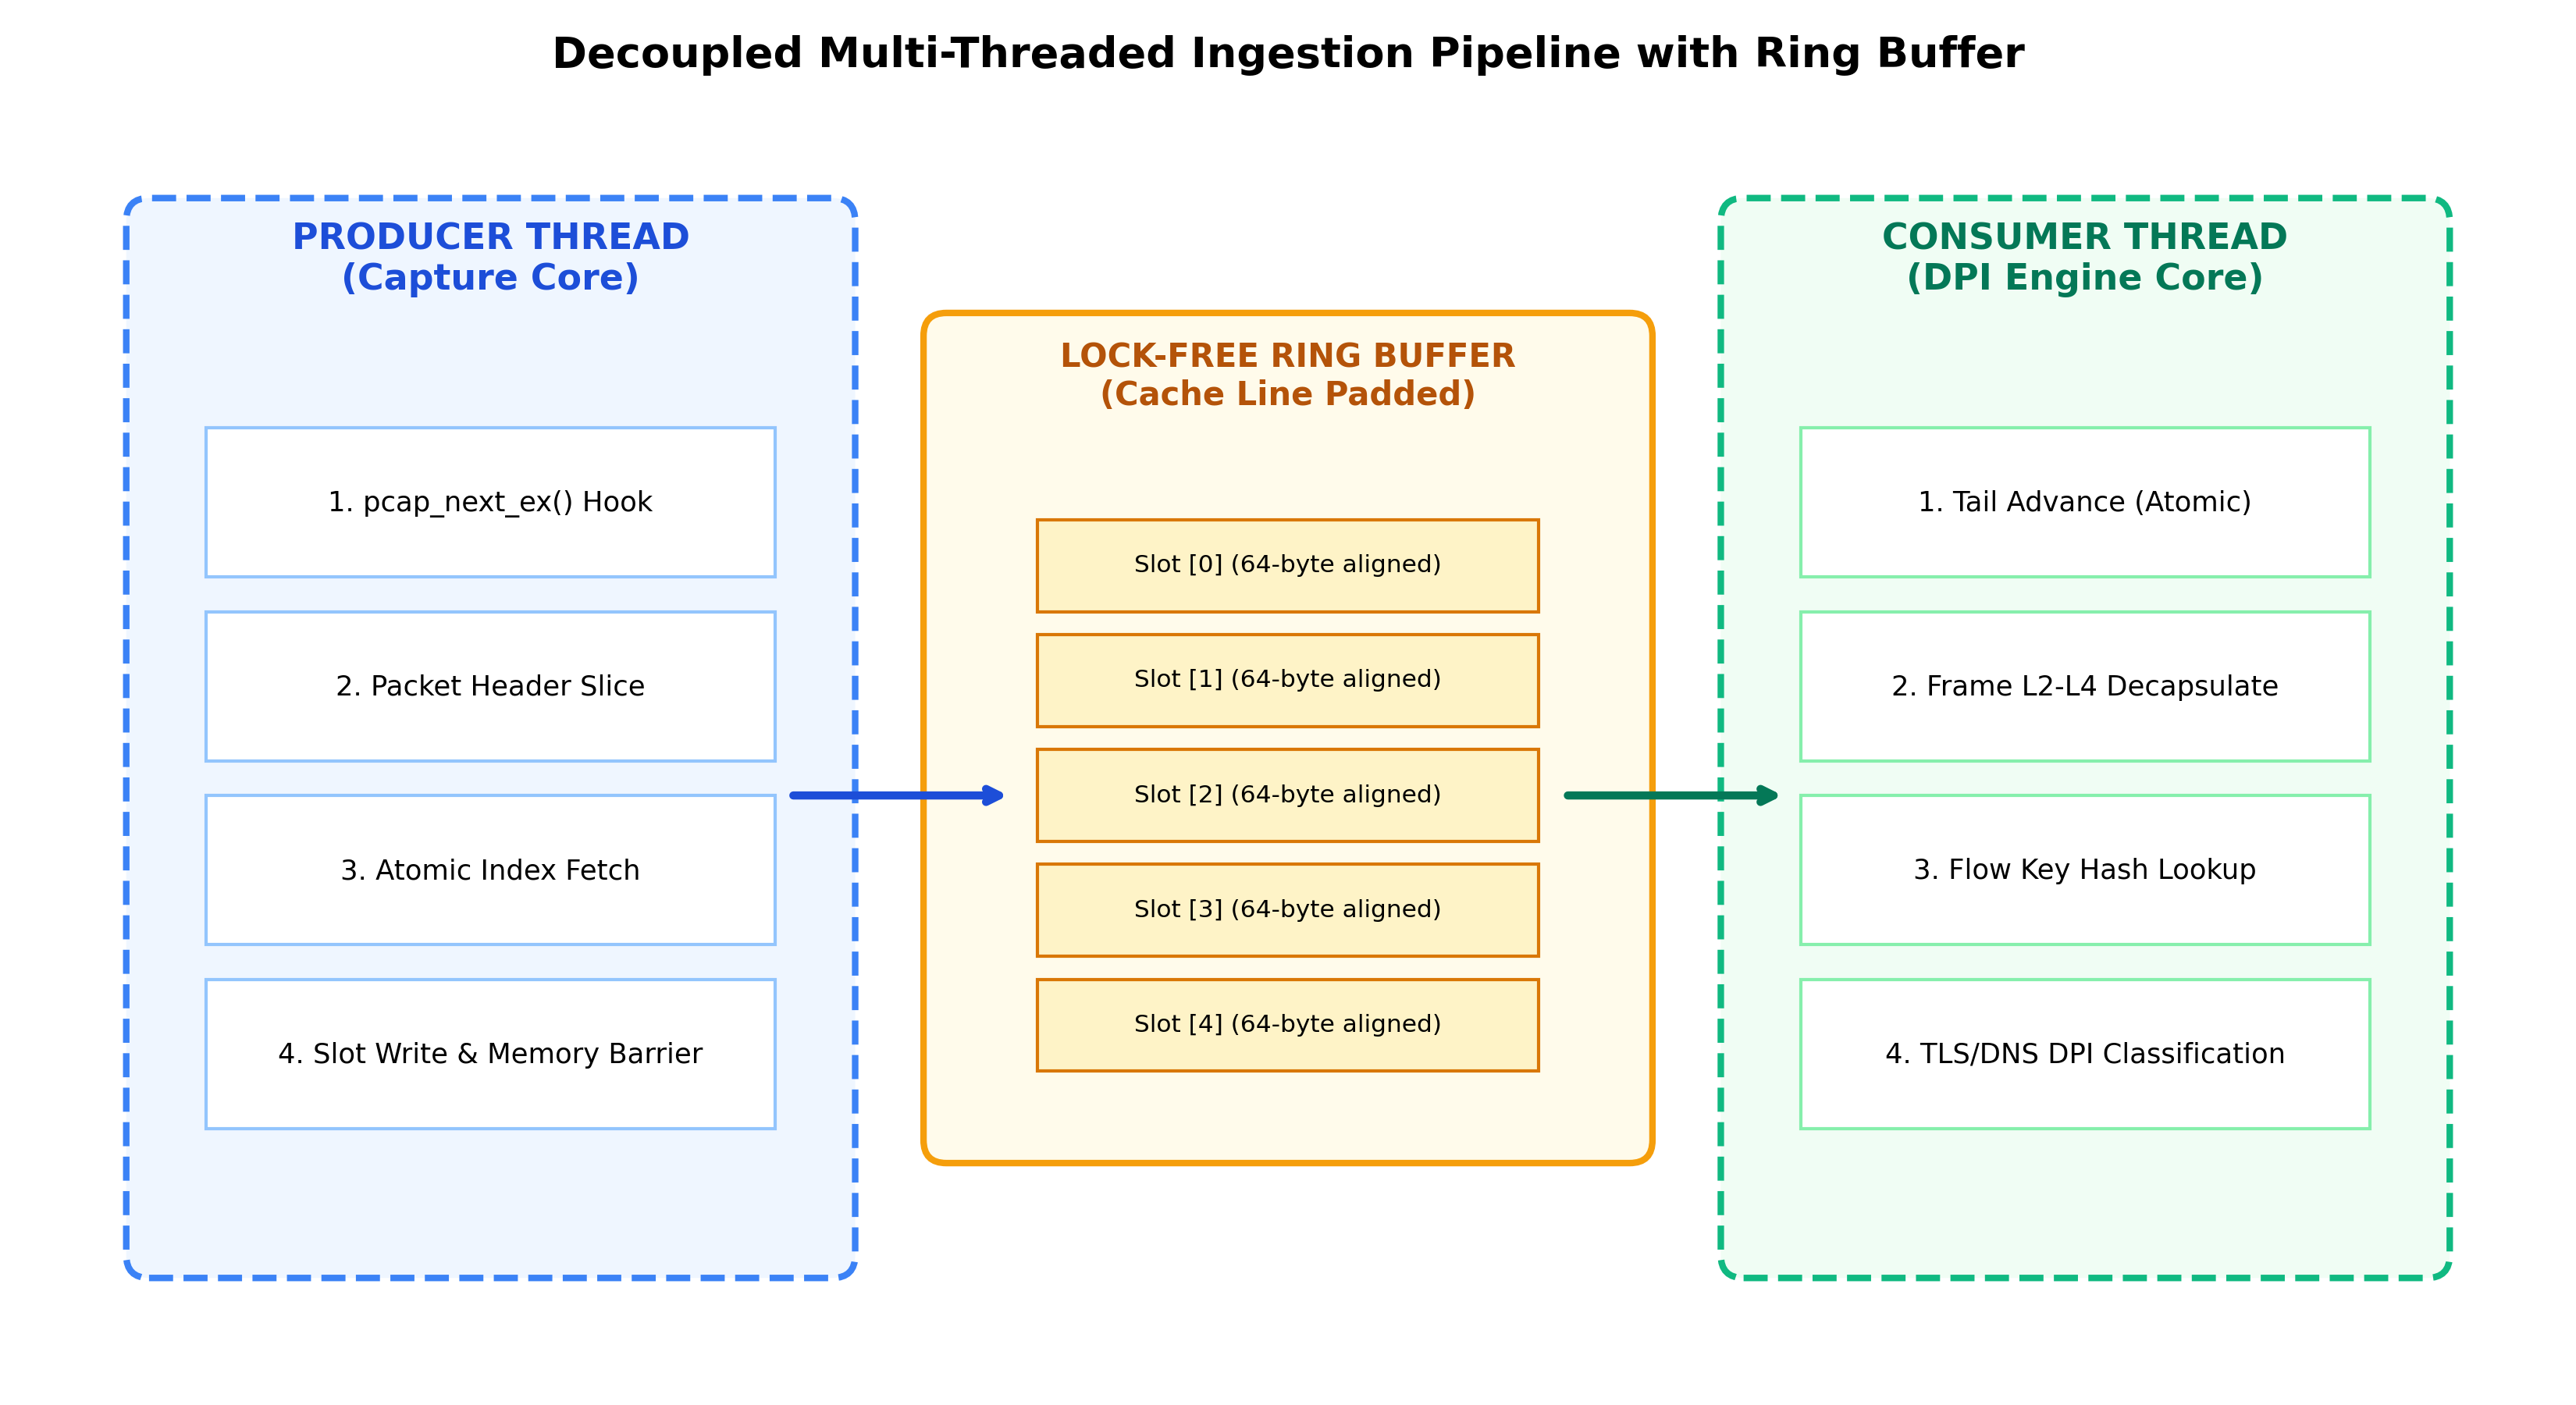
\includegraphics[width=\linewidth]{ThreadPipeline.png}
\caption{Multi-Threaded Decoupled Ingestion Pipeline with Lock-Free Ring Buffer.}
\label{fig:thread_pipeline}
\end{figure}

\subsection{Protocol Encapsulation Hierarchy}
Fig.~\ref{fig:packet_struct} illustrates the layered protocol decapsulation stack traversing Layer 2 (Ethernet II), Layer 3 (IPv4/IPv6), Layer 4 (TCP/UDP), and Layer 7 (Application payload).

\begin{figure}[htbp]
\centering
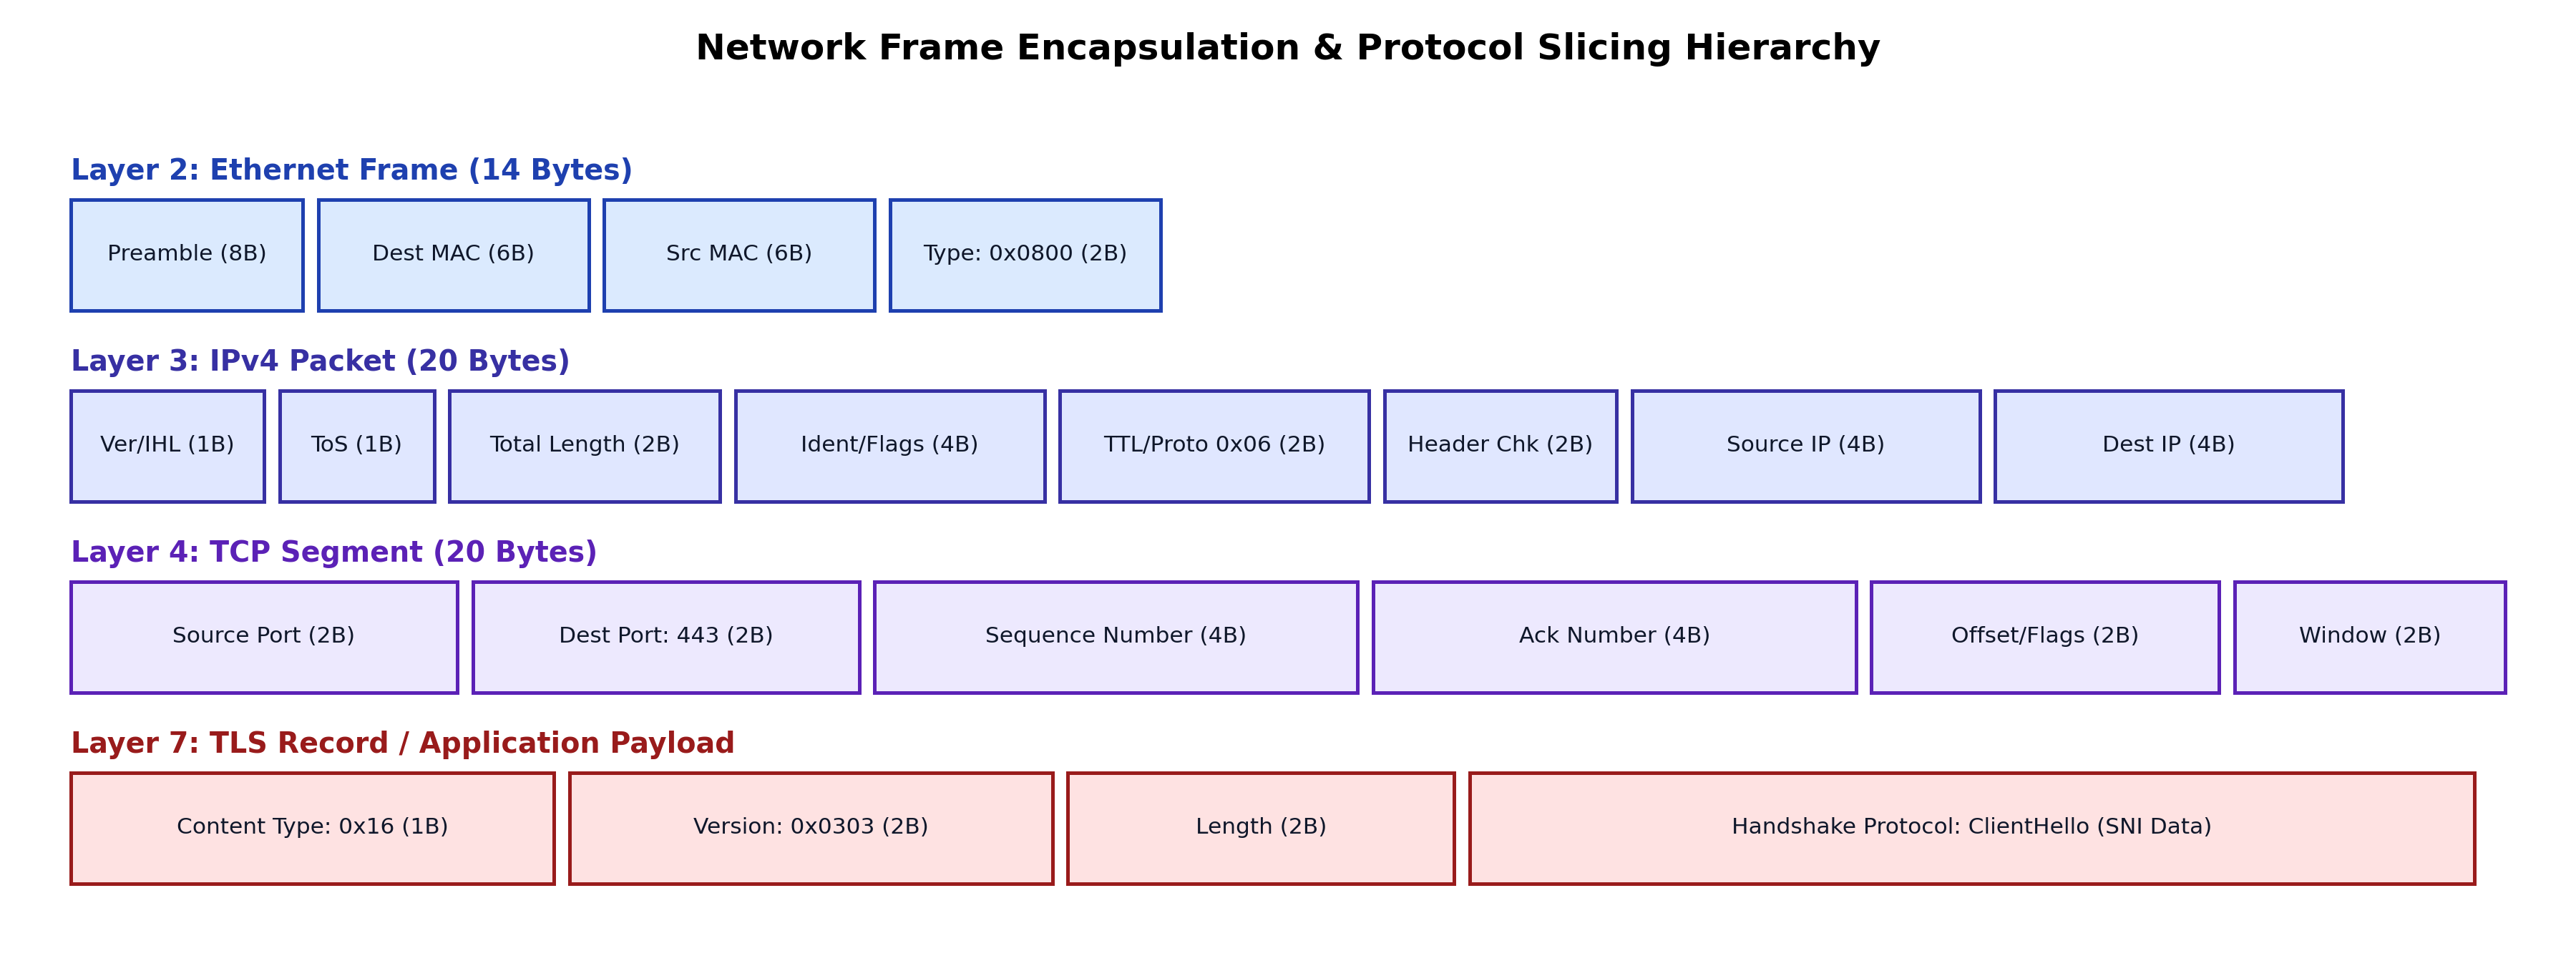
\includegraphics[width=\linewidth]{PacketStructure.png}
\caption{Protocol Decapsulation and Frame Slicing Hierarchy.}
\label{fig:packet_struct}
\end{figure}

\subsection{TLS 1.3 Cryptographic Inspection}
Under TLS 1.3, the initial \texttt{ClientHello} message is transmitted in plaintext prior to the cryptographic key exchange (Fig.~\ref{fig:tls_handshake}). DeepPacket Analyzer intercepts this record to extract the Server Name Indication (SNI) extension.

\begin{figure}[htbp]
\centering
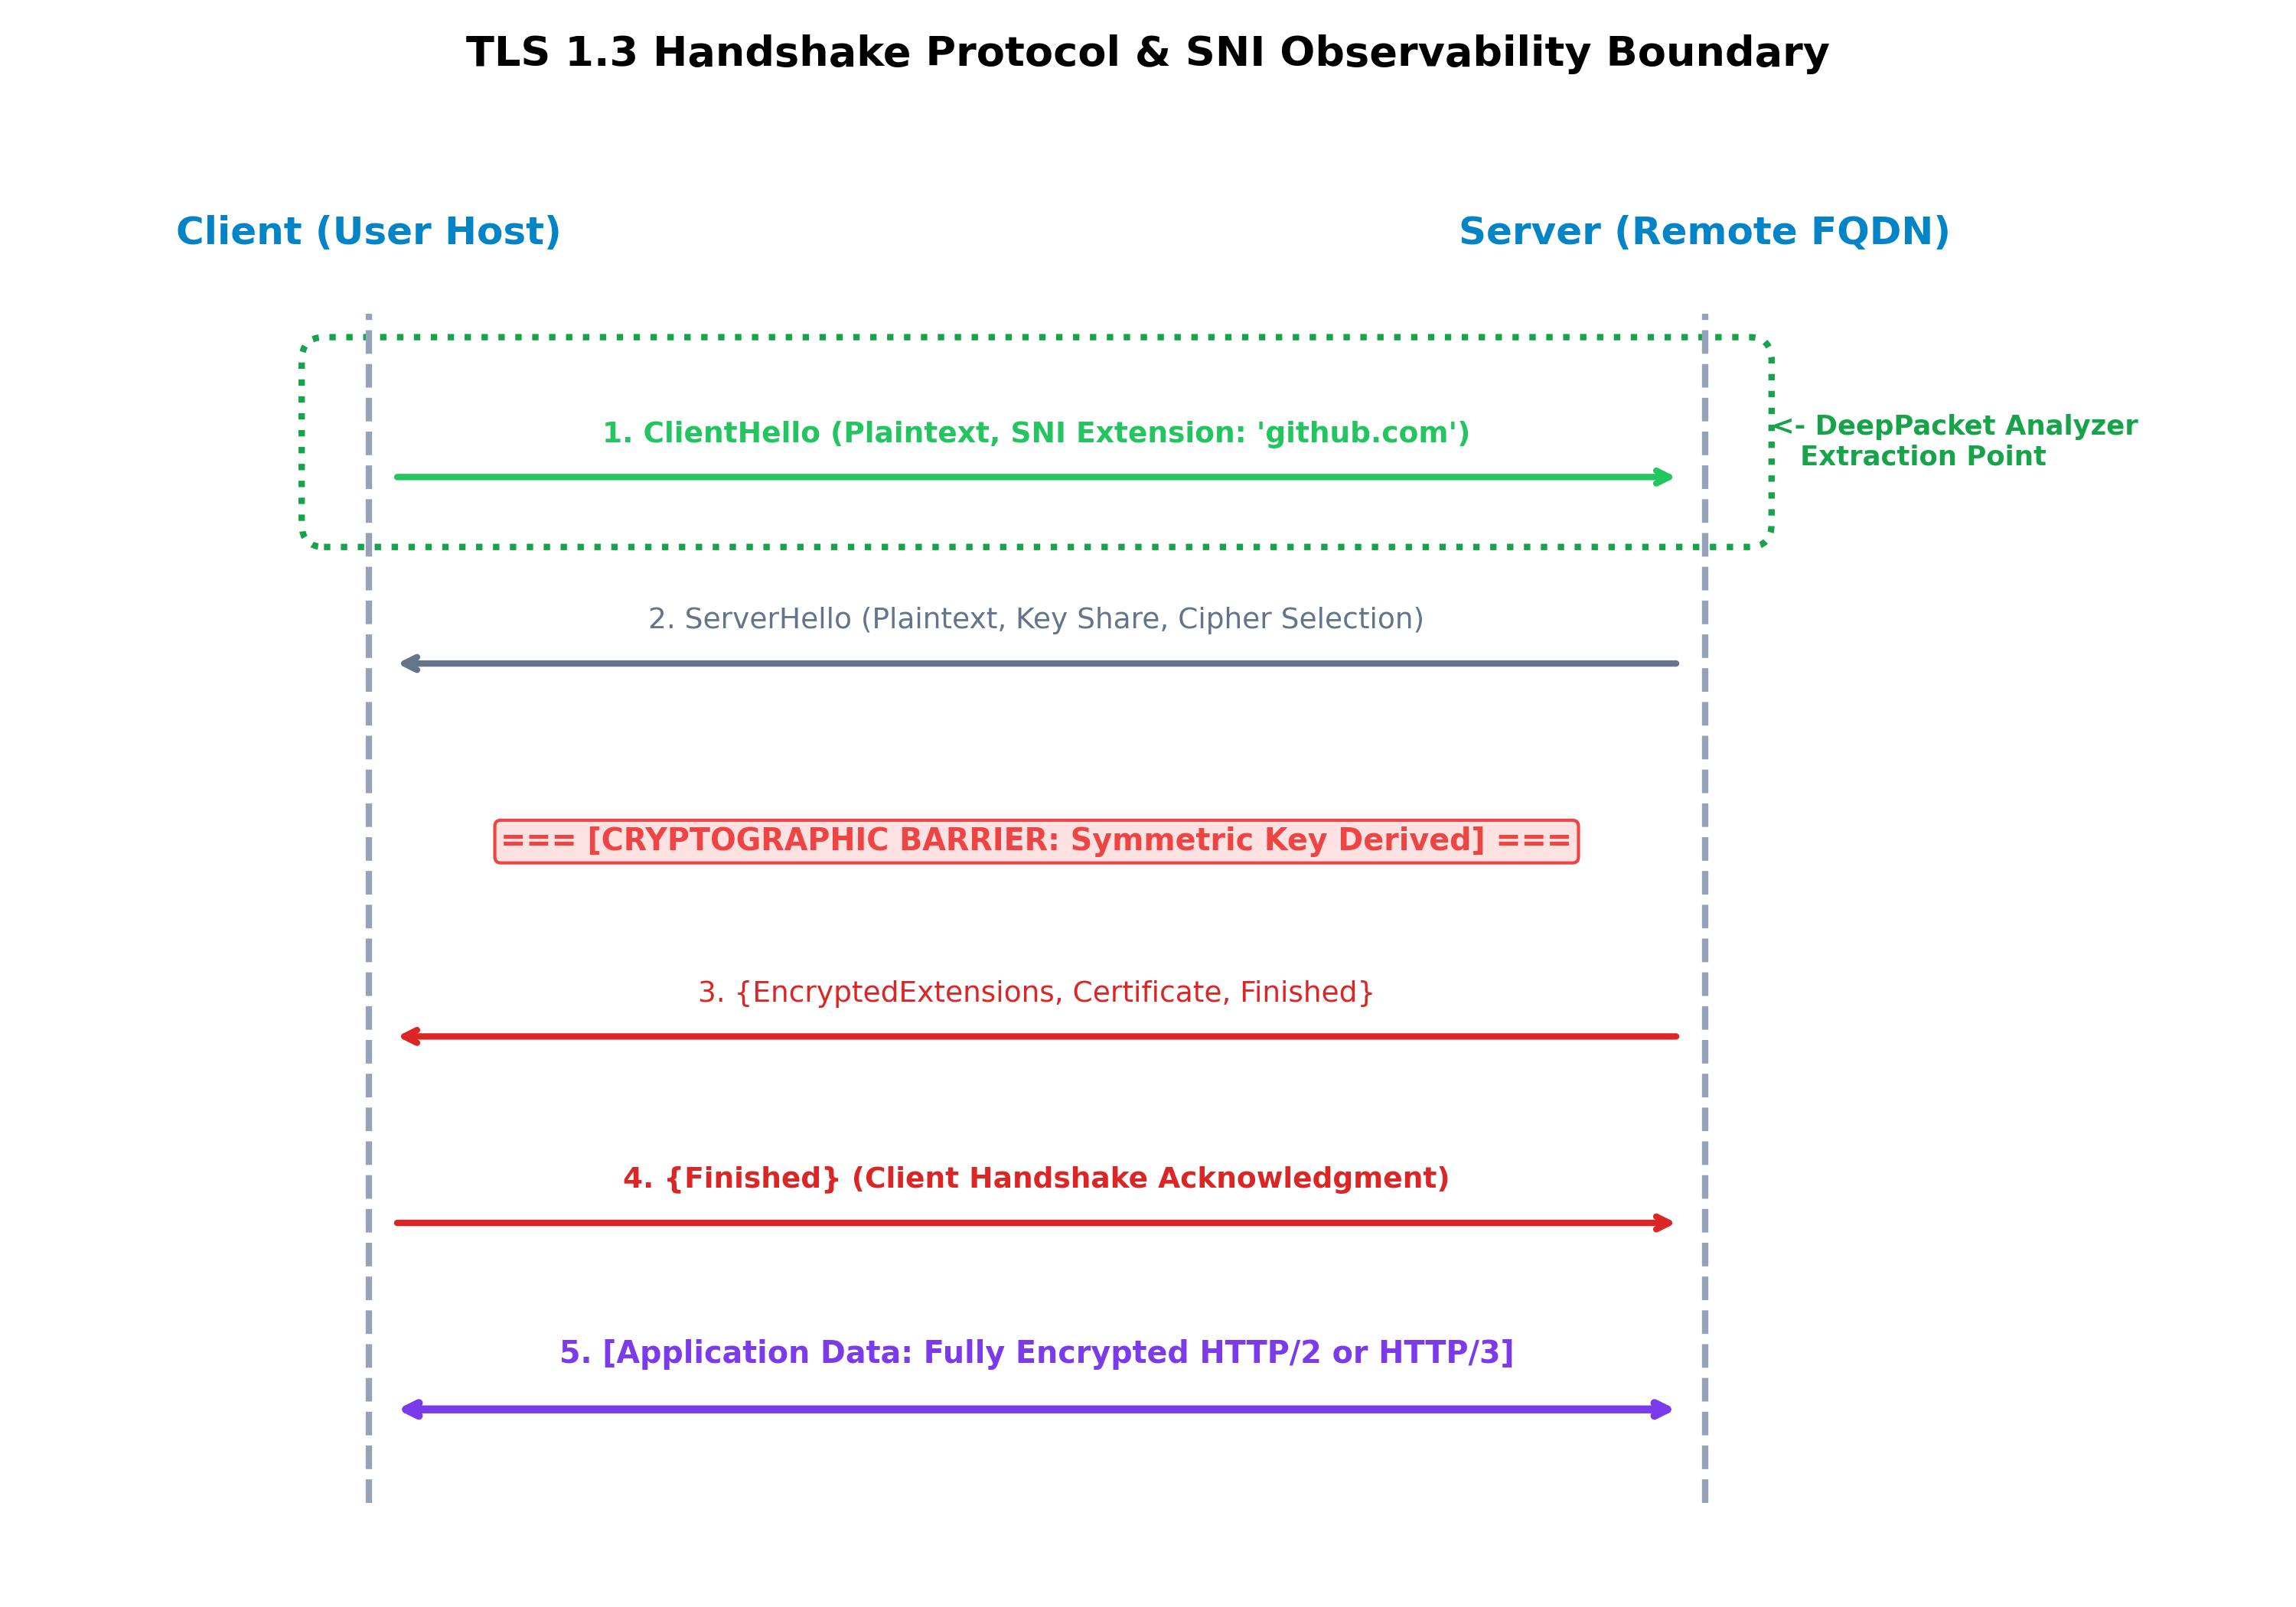
\includegraphics[width=\linewidth]{TLS_Handshake.png}
\caption{TLS 1.3 Handshake Protocol and SNI Observability Boundary.}
\label{fig:tls_handshake}
\end{figure}

The byte-level layout of the \texttt{ClientHello} frame and its SNI extension block is depicted in Fig.~\ref{fig:clienthello_struct}.

\begin{figure}[htbp]
\centering
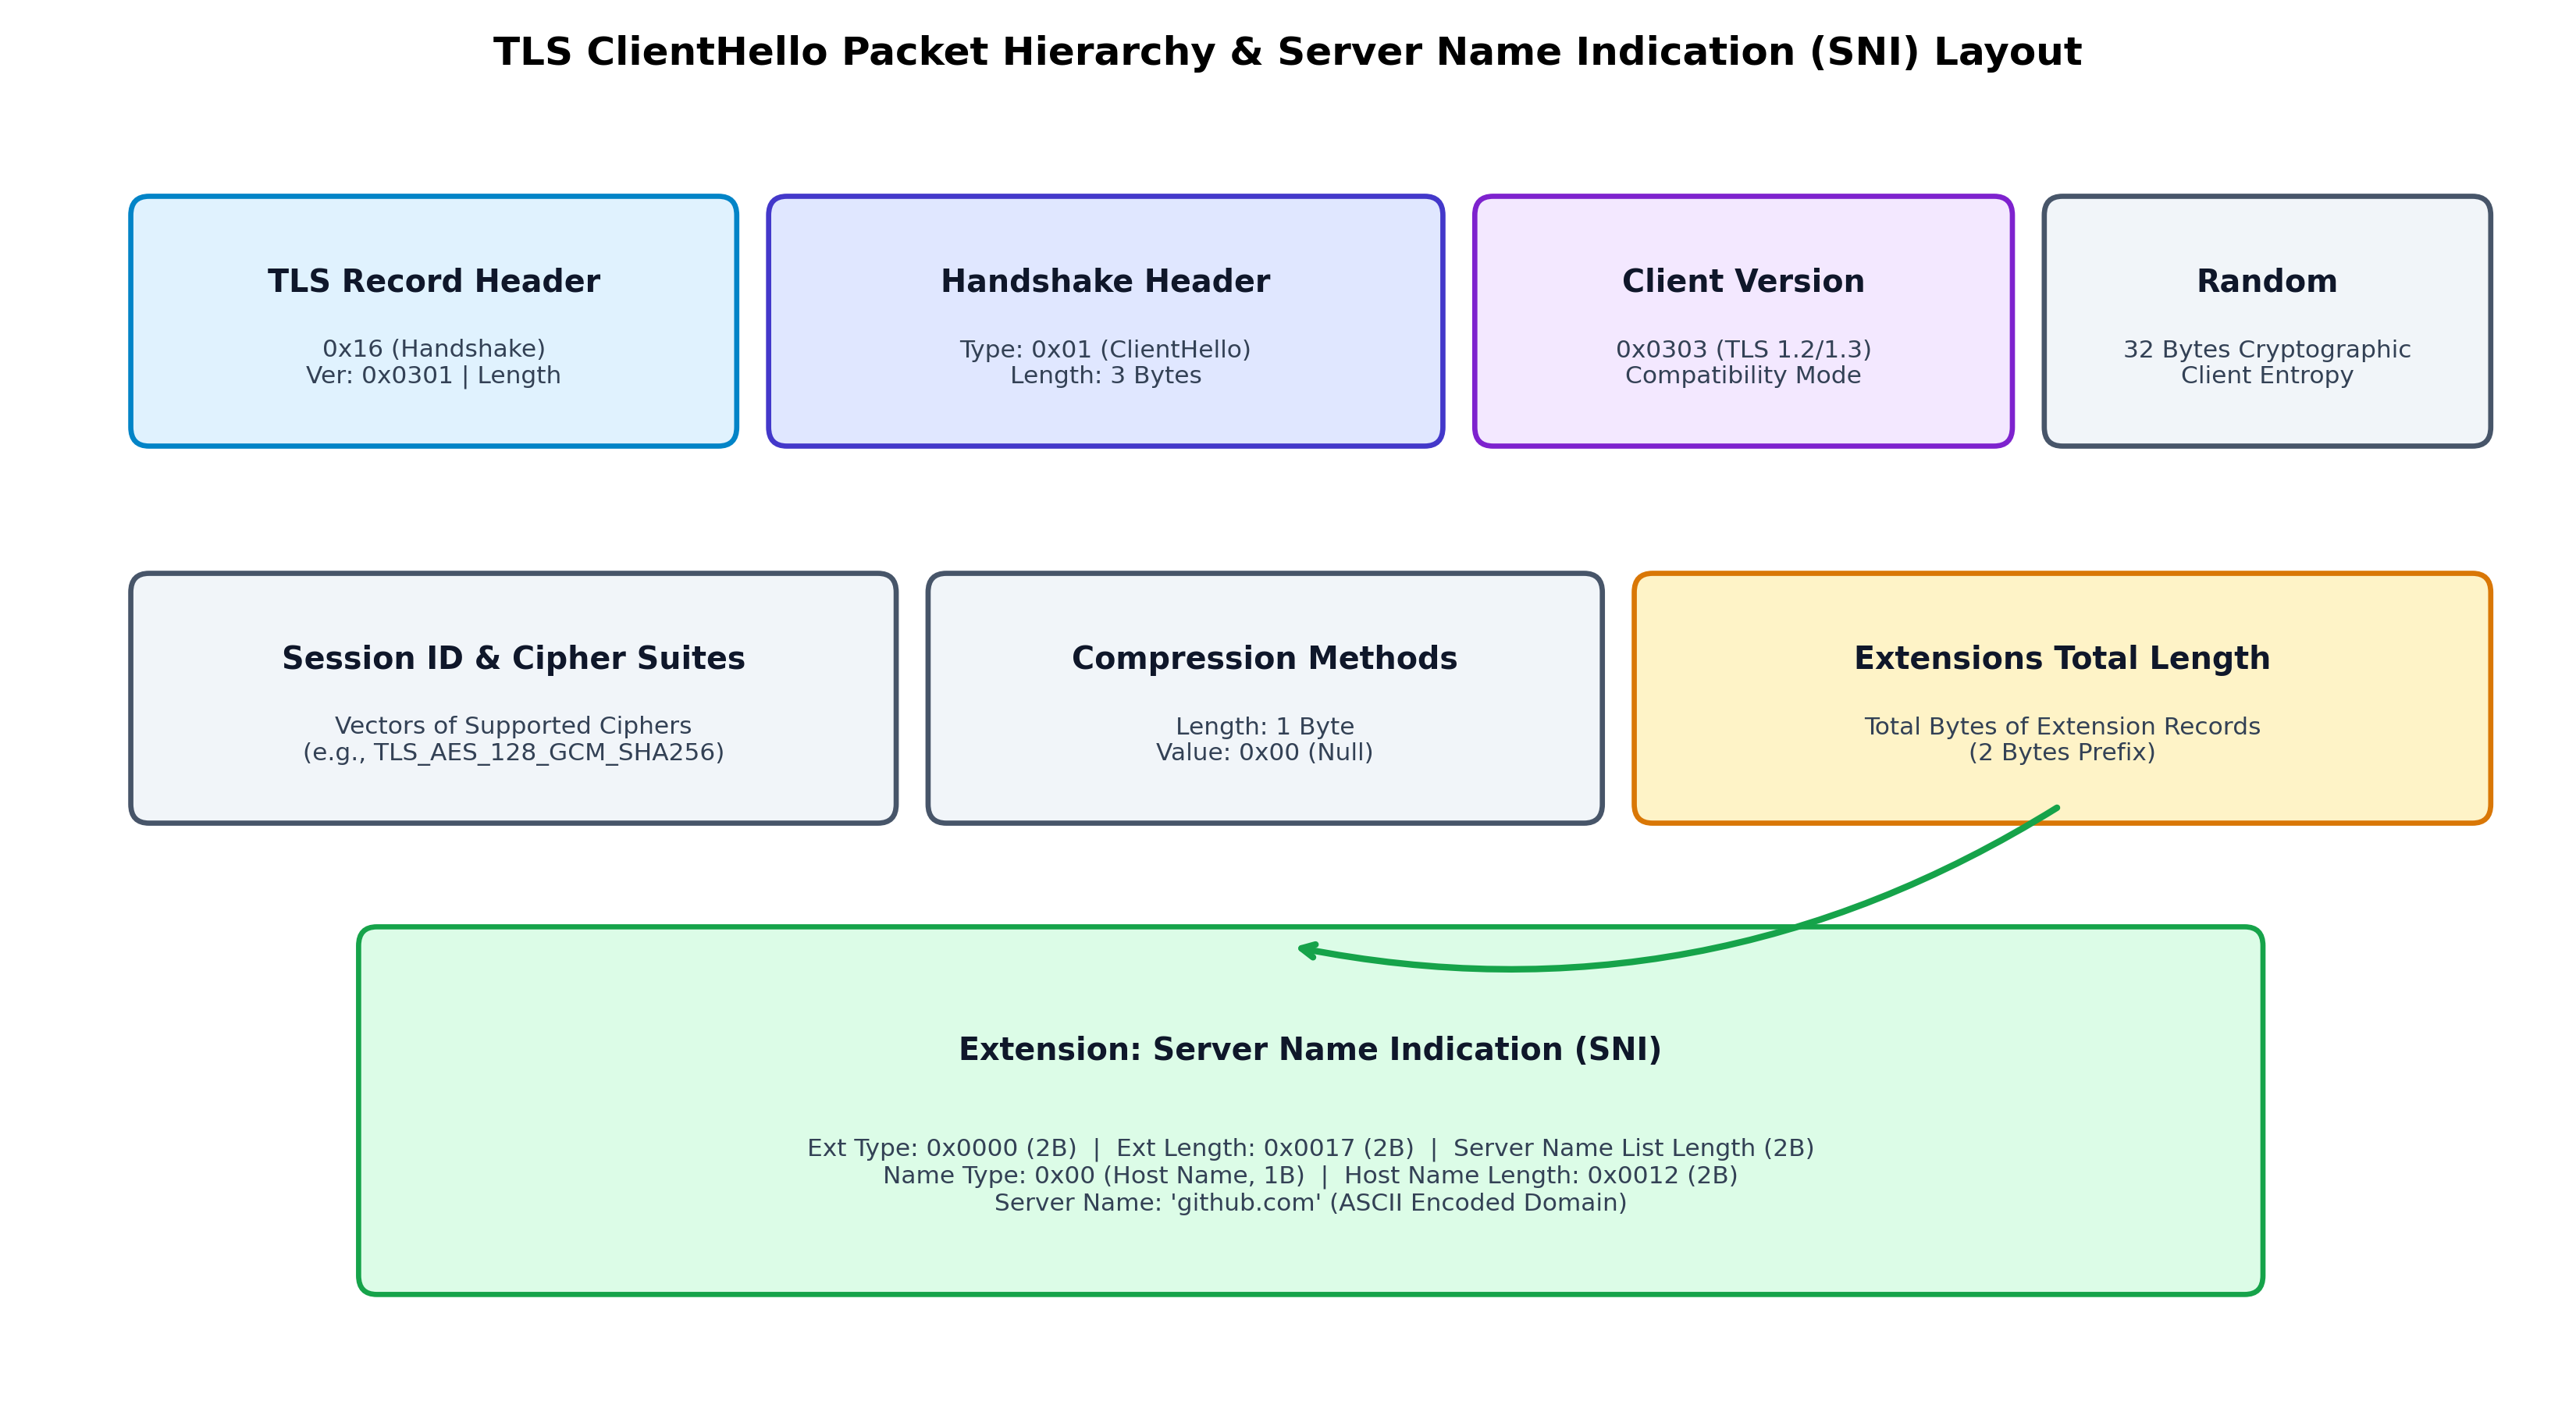
\includegraphics[width=\linewidth]{TLS_ClientHello_Structure.png}
\caption{Detailed Byte-Level Structure of TLS ClientHello and SNI Extension.}
\label{fig:clienthello_struct}
\end{figure}
